\documentclass{beamer}
\usepackage[utf8]{inputenc}

\usepackage{utopia} %font utopia imported

\usetheme{Boadilla}
\usecolortheme{default}

%------------------------------------------------------------
%This block of code defines the information to appear in the
%Title page
\title{Entrenamiento de modelos de aprendizaje profundo mediante autosupervisión}

\author
{Rubén Ezequiel Torti López}

\institute
{
  Facultad de Matemática, Astronomía, Física y Computación\\
  Universidad Nacional de Córdoba
}

\date
{Agosto 2017}

\logo{\includegraphics[height=1.0cm]{images/UNC-footer.jpg}}

%End of title page configuration block
%------------------------------------------------------------





%------------------------------------------------------------
%gets rid of bottom navigation bars
\setbeamertemplate{footline}[frame number]{}

%gets rid of bottom navigation symbols
\setbeamertemplate{navigation symbols}{}

%gets rid of footer
%will override 'frame number' instruction above
%comment out to revert to previous/default definitions
\setbeamertemplate{footline}{}
%------------------------------------------------------------





%------------------------------------------------------------
%The next block of commands puts the table of contents at the 
%beginning of each section and highlights the current section:
%
%\AtBeginSection[]
%{
%  \begin{frame}
%    \frametitle{Table of Contents}
%    \tableofcontents[currentsection]
%  \end{frame}
%}
%------------------------------------------------------------




\begin{document}
%The next statement creates the title page.
\frame{\titlepage}
%---------------------------------------------------------
%This block of code is for the table of contents after
%the title page
%\begin{frame}
%\frametitle{Table of Contents}
%\tableofcontents
%\end{frame}
%---------------------------------------------------------




\section{intro}
%---------------------------------------------------------
\begin{frame}
\frametitle{Aprendizaje automático}
Explora algoritmos cuyo objetivo es identificar patrones en conjuntos de datos.\pause
\vfill

Supera el enfoque clásico de instrucciones estáticas, tomando decisiones basadas en datos.\pause
\vfill

Tareas demasiado complejas para programarse directamente:
\vfill
\begin{examples}{Ejemplos}
\begin{itemize}
    \item Detección y verificación de caras
    \item Autos que se manejan solos 
    \item Reconocimiento del habla
    \item Diagnósticos médicos 
\end{itemize}
\end{examples}
\end{frame}
%---------------------------------------------------------





%---------------------------------------------------------
\begin{frame}
\frametitle{Aprendizaje automático}
\vfill
\begin{itemize}
    \item<1-> Supervisado 
    \item<2-> No Supervisado 
    \item<3-> Por Refuerzo 
\end{itemize}
\vfill
\end{frame}

%---------------------------------------------------------




%---------------------------------------------------------
\begin{frame}
\frametitle{Aprendizaje Supervisado}
\begin{figure}
    \centering
    \includegraphics[width=0.5\textwidth]{images/machinelearning1.pdf}
\end{figure}
\end{frame}
%---------------------------------------------------------





%---------------------------------------------------------
\begin{frame}
\frametitle{Aprendizaje No Supervisado}
\begin{figure}
    \centering
    \includegraphics[width=0.5\textwidth]{images/machinelearning2.pdf}
\end{figure}
\end{frame}
%---------------------------------------------------------





\section{marco}
%---------------------------------------------------------
\begin{frame}
\frametitle{Modelos lineales}
\begin{itemize}
    \item Clasificación
    \item Función de costo y SGD 
\end{itemize}
\end{frame}
%---------------------------------------------------------





%---------------------------------------------------------
\begin{frame}
\frametitle{Modelos no lineales}
\begin{itemize}
    \item Redes neuronales
    \item Regularizacion
    \item Backpropagation
    \item Preprocesamiento de datos
    \item Transferencia de aprendizaje
    \item Redes convolucionales
\end{itemize}
\end{frame}
%---------------------------------------------------------





%---------------------------------------------------------
\begin{frame}
\frametitle{Redes Convolucionales}
Notación:
\begin{itemize}
    \item C\(k\): capa convolucional con \(k\) filtros cuadrados
    \item F\(k\): capa completamente conectada (FC) con salida de dimensión \(k\)
    \item P: \textit{Pooling}. Usualmente \textit{MAX Pooling}
    \item D: \textit{Dropout}
    \item Op para la capa de salida
\end{itemize}
\end{frame}
%---------------------------------------------------------





%---------------------------------------------------------
\begin{frame}
\frametitle{Redes Convolucionales}
\begin{figure}
    \centering
    \includegraphics[width=\textwidth]{images/net_example.pdf}
\end{figure}
\begin{itemize}
    \item Arquitectura de red convolucional: C96-P-C256-F500-Op.
    \item Luego de cada capa convolucional se utilizan unidades ReLU y luego de cada capa completamente conectada se agrega una capa de \textit{Dropout}.
\end{itemize}
\end{frame}
%---------------------------------------------------------





\section{pretext}
%---------------------------------------------------------
\begin{frame}
\frametitle{Entrenamiento mediante tareas de pretexto}
Tareas de pretexto \\\vfill

No son útiles en si mismas, pero sirven para aprender representaciones generales que puedan ser aplicadas a otro problema.\\\vfill
	
\begin{itemize}
    \item reconstrucción de la imagen de entrada
    \item predicción de píxeles en una secuencia de video 
    \item ordenamiento temporal de cuadros de videos
    \item ordenamiento parches en imágenes estáticas
\end{itemize}\\
\vfill

Anotaciones fáciles de obtener e incluso a partir del mismo conjunto de datos. \\
\vfill
La hipótesis es que el modelo aprenderá características de alto nivel para poder realizar su tarea.
\vfill
\end{frame}
%---------------------------------------------------------





%---------------------------------------------------------
\begin{frame}
\frametitle{Entrenamiento mediante tareas de pretexto}
Redes siamesas\\
\vfill
Sea \(G_W(x)\) una familia de funciones con parámetros \(W\)\\
\vfill
	
Queremos encontrar \(W\) tal que para una medida de similitud \(D\),\\

\vfill
	
\(D(G_W(x_1), G_W(x_2))\) sea pequeña sii \(x_1\) y \(x_2\) pertenecen a la misma categoría y
grande en caso contrario.\pause 
\vfill
	
	
¿Cómo optimizar los parámetros \(W\)?\\\pause
\vfill

Estableciendo una función de costo que minimice \(D(G_W(x_1), G_W(x_2))\)
\end{frame}
%---------------------------------------------------------





%---------------------------------------------------------
\begin{frame}
\frametitle{Entrenamiento mediante tareas de pretexto}
Redes siamesas\\
\begin{figure}
    \centering
    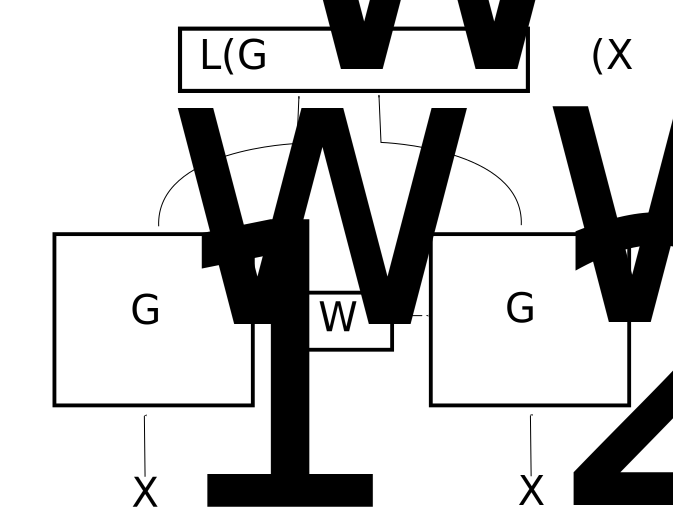
\includegraphics[width=0.5\textwidth]{images/siamese-diagram.pdf}
\end{figure}
\end{frame}
%---------------------------------------------------------





%---------------------------------------------------------
\begin{frame}
\frametitle{Herramientas}
\begin{figure}
    \centering
    \includegraphics[width=0.6\textwidth]{images/tools.png}
\end{figure}
\end{frame}
%---------------------------------------------------------





%---------------------------------------------------------
\begin{frame}
\frametitle{\textit{Slow Feature Analysis}}

Técnica de aprendizaje no supervisado:
\begin{itemize}
    \item \textit{features} cambian poco en una ventana de tiempo pequeña \pause
	\end{itemize}

	Sean \(x_{t_1}\) y \(x_{t_2}\) representaciones de imágenes en tiempos \(t_1\) y \(t_2\)\\
Sea \(D\) una medida de similitud. Podemos definir una función de costo:

\begin{equation}
L(x_{t_1}, x_{t_2}, W) = \begin{cases}
                           D(x_{t_1}, x_{t_2}),& \text{si} |t_1 - t_2| \leq T \\ 
                           1 - \max{(0, m - D(x_{t_1}, x_{t_2}))},& \text{si} |t_1 - t_2| > T
                         \end{cases}
\end{equation}

\(W\) son los parámetros compartidos de las redes siamesas\\
\(m\) es el margen mínimo que debe separar a las representaciones distintas.
\end{frame}
%---------------------------------------------------------


%---------------------------------------------------------
\begin{frame}
\frametitle{\textit{Slow Feature Analysis}}
\begin{figure}
    \centering
    \includegraphics[width=0.8\textwidth]{images/example_contrastiveloss.png}
\end{figure}
\end{frame}
%---------------------------------------------------------




%---------------------------------------------------------
\begin{frame}
\frametitle{Automovimiento}

¿Podemos predecir cuando dos fotos son la misma a pesar haber sufrido alguna transformación?\\

\vfill

\begin{itemize}
    \item tarea de clasificación donde el objetivo es predecir la transformación 
\end{itemize}

\vfill

\begin{block}{Información Odométrica}
Información sobre el cambio de posición respecto a un punto inicial.
\end{block}
\vfill

¿Puede un agente móvil valerse de la información obtenida de su propio movimiento para
supervisar el aprendizaje de buenas representaciones visuales de su
entorno?
\end{frame}
%---------------------------------------------------------





%---------------------------------------------------------
\begin{frame}
\frametitle{Automovimiento}

¿Como sabemos si cuando son buenas representaciones?\\\pause

\vfill
\begin{enumerate}
    \item la capacidad de poder realizar múltiples tareas visuales
    \item la habilidad de poder aprender nuevas tareas visuales basándose en pocos ejemplos.
\end{enumerate}\pause
\vfill

\begin{block}{}
El problema de relacionar los estímulos visuales con el automovimiento puede ser establecido como el problema de predecir las transformaciones de la cámara en pares de imágenes a lo largo del movimiento de la misma
\end{block}
\vfill
\end{frame}
%---------------------------------------------------------





%---------------------------------------------------------
\begin{frame}
\frametitle{Información odométrica para entrenar redes siamesas}
\begin{itemize}
    \item Tarea de clasificación: predecir transformaciones en \(X, Y, Z\)
    \item Transformaciones en espacio continuo 
    \item 3 clasificadores con categorías discretizadas
\end{itemize}
\end{frame}
%---------------------------------------------------------





\section{Experimentos}
%---------------------------------------------------------
\begin{frame}
\frametitle{Experimentos - Diseño}
\begin{itemize}
    \item Particionado del conjunto de entrenamiento
    \item Hiperparámetros
    \item Preentrenamiento inicial
    \item Transferencia de aprendizaje
    \item Chequeo de métricas
\end{itemize}
\end{frame}
%---------------------------------------------------------





%---------------------------------------------------------
\begin{frame}
\frametitle{Experimentos - Prueba de concepto: MNIST}
Conjunto de datos de dígitos manuscritos
\vfill
Pares artificiales con traslaciones en X e Y, rotaciones en Z
\vfill
\begin{figure}
\centering
\resizebox{.9\linewidth}{!}{
\begin{tabular}{cccccc}
\includegraphics[width = 1.5in]{./images/mnist/a1.png} &
\includegraphics[width = 1.5in]{./images/mnist/a.png} &
\includegraphics[width = 1.5in]{./images/mnist/b1.png} &
\includegraphics[width = 1.5in]{./images/mnist/b.png} &
\includegraphics[width = 1.5in]{./images/mnist/c.png} &
\includegraphics[width = 1.5in]{./images/mnist/c1.png}\\
\end{tabular}
}
\label{fig:mnist-sample}
\end{figure}
\vfill

\end{frame}
%---------------------------------------------------------





%---------------------------------------------------------
\begin{frame}[plain]
\frametitle{Experimentos - Prueba de concepto: MNIST}
\begin{figure}
    \centering
    \includegraphics[width=0.9\textwidth]{images/siamese-example.pdf}
\end{figure}
\end{frame}
%---------------------------------------------------------






%---------------------------------------------------------
\begin{frame}
\frametitle{Experimentos - Prueba de concepto: MNIST}
\begin{itemize}
    \item BCNN: C96-P-C256-P, TCNN: F1000-D-Op.
    \item 40K iteraciones, lr inicial: 0.01, márgenes 10 y 100 para SFA
    \item mini-batch: 125, total de 5 millones de pares de imágenes
    \item \textit{cross-validation}: partición en entrenamiento-validación
    \item Transferencia de aprendizaje: BCNN + F500-D-F10-Softmax. lr: 0 en capas convolucionales
\end{itemize}
\vfill
\begin{block}{Métricas}
Accuracy, Función de costo durante entrenamiento
\end{block}
\end{frame}
%---------------------------------------------------------





%---------------------------------------------------------
\begin{frame}
\frametitle{Experimentos - Prueba de concepto: MNIST}
\begin{table}
\centering
\begin{tabular}{l|rrrr}
\hline
\multicolumn{1}{r}{}
& \multicolumn{4}{c}{datos entrenamiento}
& \multicolumn{1}{l}{Método}
& \multicolumn{1}{r}{100}
& \multicolumn{1}{r}{300}
& \multicolumn{1}{r}{1000}
& \multicolumn{1}{r}{10000} \\ \cline{1-5}
\hline
Desde cero & 0.42 & 0.70 & 0.82 & 0.97\\
SFA(m=10) & 0.52 & 0.71 & 0.77 & 0.82\\
SFA(m=100) & 0.58 & 0.73 & 0.80 & 0.88\\
Automovimiento & 0.75 & 0.90 & 0.92 & 0.99\\
\hline
\end{tabular}
\end{table}
\end{frame}
%---------------------------------------------------------





%---------------------------------------------------------
\begin{frame}
\frametitle{Experimentos - KITTI}
\vfill
11 secuencias que registran el movimiento de un automóvil en una ciudad\vfill
\begin{figure}
\centering
\resizebox{.9\linewidth}{!}{
\includegraphics[width = 1.5in]{./images/kitti/original.png} &
}
\end{figure}
\vfill
\begin{itemize}
    \item matrices de rotación Las transformaciones en X, Y y Z en base a las matrices de rotación provistas por los creadores del conjunto de datos.
    \item Para las rotaciones en el eje Y se calculó el ángulo de Euler correspondiente al cambio entre dos \textit{frames}.
    \item Discretización de traslaciones y rotaciones en categorías
\end{itemize}
\vfill
\end{frame}
%---------------------------------------------------------





%---------------------------------------------------------
\begin{frame}
\frametitle{KITTI - Pares de entrenamiento}
\begin{figure}
\centering
\resizebox{.9\linewidth}{!}{
\begin{tabular}{cccccc}
\includegraphics[width = 1.5in]{./images/kitti/a.png} &
\includegraphics[width = 1.5in]{./images/kitti/a1.png} &
\includegraphics[width = 1.5in]{./images/kitti/b.png} &
\includegraphics[width = 1.5in]{./images/kitti/b1.png} &
\includegraphics[width = 1.5in]{./images/kitti/c.png} &
\includegraphics[width = 1.5in]{./images/kitti/c1.png}\\
\end{tabular}
}
\label{fig:kitti-sample}
\end{figure}
\vfill
\begin{itemize}
    \item Clasificación, 20 clases por eje
    \item Automovimiento: cuadros separados a lo sumo por 7 cuadros intermedios.
    \item SFA: ±7 cuadros considerados cercanos
    \item Se extrayeron parches aleatorios de \(227 \times 227\)
\end{itemize}
\vfill
\end{frame}
%---------------------------------------------------------





%---------------------------------------------------------
\begin{frame}[plain]
\frametitle{KITTI - Entrenamiento}
\vfill
\begin{itemize}
    \item BCCN: C96-P-C256-P-C384-C384-C256-P. La TCNN fue definida como C256-C128-F500-D-Op
    \item Pre-entrenamiento 60K iteraciones con \textit{mini batch} de 125 imágenes,
    \item tasa de aprendizaje inicial de \(0.001\), reducida en un factor de 2 cada 20K iteraciones.
    \item transferencia de aprendizaje: 10K iteraciones, lr constante 0.001. Para diferenciar los distintos
\end{itemize}\pause
\vfill
\begin{block}{Baseline}
Se entrenó AlexNet con el conjunto de datos ILSVRC'12 desde cero utilizando 20 y 1000 imágenes por clase (ALEX-20 y ALEX-1000)\\
Las redes siamesas fueron entrenadas con aproximadamente 20K pares de imágenes.
\end{block}\pause
\vfill
\end{frame}
%---------------------------------------------------------





%---------------------------------------------------------
\begin{frame}
\frametitle{Experimentos - KITTI + SUN395}
397 categorías de paisajes interiores y exteriores\vfill
\textit{Cross-validation} con 3 particiones\vfill
\begin{figure}
\centering
\resizebox{.7\linewidth}{!}{
\begin{tabular}{cccc}
\includegraphics[width = 1.5in]{./images/sun397/mountain_snowy.jpg} &
\includegraphics[width = 1.5in]{./images/sun397/oilrig.jpg} &
\includegraphics[width = 1.5in]{./images/sun397/nuclear_power_plant.jpg} &
\includegraphics[width = 1.5in]{./images/sun397/rock_arch.jpg} \\
\includegraphics[width = 1.5in]{./images/sun397/subway_station.jpg} &
\includegraphics[width = 1.5in]{./images/sun397/kennel.jpg} &
\includegraphics[width = 1.5in]{./images/sun397/pilothouse.jpg} &
\includegraphics[width = 1.5in]{./images/sun397/abbey.jpg} \\
\end{tabular}
}
\end{figure}
\end{frame}
%---------------------------------------------------------





%---------------------------------------------------------
\begin{frame}
\frametitle{Experimentos - KITTI + SUN395}
Preentrenamiento: automovimiento, SFA y pesos aleatorios.
\vfill
Transferencia de aprendizaje con SUN395 con 5 y 20 elementos por categoría.
\vfill
Calidad de las representaciones: \textit{Softmax} para cada capa\pause
\vfill
Accuracy:
\begin{table}
\centering
\resizebox{\textwidth}{!}{
\begin{tabular}{l|r|r|ccccc|r|ccccc}
\hline
\multicolumn{1}{l}{Método}
& \multicolumn{1}{r}{\#preentr.}
& \multicolumn{1}{r}{\#finet.}
& \multicolumn{1}{c}{L1}
& \multicolumn{1}{c}{L2}
& \multicolumn{1}{c}{L3}
& \multicolumn{1}{c}{L4}
& \multicolumn{1}{c}{L5}
& \multicolumn{1}{r}{\#finet.}
& \multicolumn{1}{c}{L1}
& \multicolumn{1}{c}{L2}
& \multicolumn{1}{c}{L3}
& \multicolumn{1}{c}{L4}
& \multicolumn{1}{c}{L5} \\ \cline{1-14}
\hline

ALEX-1000 & 1M & 5 & 3.73 & 5.07 & 5.07 & 8.53 & 10.40 & 20 & 9.07 & 12.53 & 16.27 & 17.60 & 10.67\\
ALEX-20 & 20K & 5 & 2.93 & 1.87 & 3.73 & 5.07 & 3.20 & 20 & 6.13 & 5.33 & 5.33 & 4.53 & 5.07\\
KITTI-SFA & 20.7K & 5 & 2.13 & 3.20 & 2.40 & 1.60 & 1.87 & 20 & 4.53 & 3.73 & 2.13 & 2.40 & 2.93\\
KITTI-EGO & 20.7K & 5 & 2.93 & 1.87 & 3.20 & 5.87 & 1.33 & 20 & 6.67 & 7.47 & 9.87 & 9.33 & 4.00\\

\hline
\end{tabular}
}
\end{table}
\vfill
\end{frame}
%---------------------------------------------------------





%---------------------------------------------------------
\begin{frame}
\frametitle{Experimentos - KITTI + ImageNet}
Conjunto de datos ILSVRC'12, 1000 categorías
\begin{figure}
\centering
\resizebox{.75\linewidth}{!}{
\begin{tabular}{cccc}
\includegraphics[width = 1.5in]{./images/imagenet/n01531178_108.JPEG} &
\includegraphics[width = 1.5in]{./images/imagenet/n01675722_126.JPEG} &
\includegraphics[width = 1.5in]{./images/imagenet/n01753488_177.JPEG} &
\includegraphics[width = 1.5in]{./images/imagenet/n01773797_48.JPEG} \\
\includegraphics[width = 1.5in]{./images/imagenet/n02859443_1229.JPEG} &
\includegraphics[width = 1.5in]{./images/imagenet/n03000134_789.JPEG} &
\includegraphics[width = 1.5in]{./images/imagenet/n03017168_743.JPEG} &
\includegraphics[width = 1.5in]{./images/imagenet/n03085013_2149.JPEG} \\
\end{tabular}
}
\end{figure}
\vfill
Se crearon conjuntos de datos con 1 5, 10, 20 y 1000 imágenes por categoría
\vfill
\end{frame}
%---------------------------------------------------------





%---------------------------------------------------------
\begin{frame}
\frametitle{Experimentos - KITTI + ImageNet}

Preentrenamiento con automovimiento, SFA y pesos aleatorios.\pause
\vfill
Transferencia de aprendizaje con ImageNet.\pause
\vfill

Accuracy:
\begin{table}
\centering
\begin{tabular}{l|ccccc}
\hline
\multicolumn{1}{l}{Método}
& \multicolumn{1}{c}{1}
& \multicolumn{1}{c}{5}
& \multicolumn{1}{c}{10}
& \multicolumn{1}{c}{20}
& \multicolumn{1}{c}{1000} \\ \cline{1-6}
\hline

KITTI-EGO & 0.49 & 1.27 & 2.14 & 4.13 & 20.8\\
KITTI-SFA & 0.35 & 0.75 & 1.34 & 2.64 & 11.83\\
ALEXNET & 0.45 & 0.95 & 1.91 & 3.69 & 18.35\\

\hline
\end{tabular}
\end{table}
\end{frame}
%---------------------------------------------------------





%---------------------------------------------------------
\begin{frame}
\frametitle{Conclusiones}
\begin{itemize}
    \item \textit{automovimiento} permite obtener  resultados equiparables al estado del arte.
    \item Anotaciones de automovimiento fáciles de obtener. 
    \item Bajo la misma cantidad de imágenes de preentrenamiento, \textit{automovimiento} equipara a técnicas supervisadas de clasificación.
\end{itemize}
\end{frame}
%---------------------------------------------------------





%---------------------------------------------------------
\begin{frame}
\frametitle{Trabajo a Futuro}
\begin{itemize}
    \item Probar otras variantes: arquitecturas de redes, conjuntos de datos
    \item ¿Puede el \textit{automovimiento} aplicarse a otros dominios?
    \item Evaluar la utilidad de otras tareas de pretexto
\end{itemize}
\end{frame}
%---------------------------------------------------------





%---------------------------------------------------------
\begin{frame}
\frametitle{}
\vfill
	¿Preguntas?
\vfill
\end{frame}
%---------------------------------------------------------





%---------------------------------------------------------
\begin{frame}
\frametitle{}
\vfill
    Gracias!
\vfill
\end{frame}
%---------------------------------------------------------
\end{document}
